\documentclass[11pt]{article}

\usepackage[utf8]{inputenc}
\usepackage{amsmath, amssymb, amsthm}
\usepackage[inkscapeformat=pdf]{svg}
\usepackage{placeins}
\usepackage{tabularx}
\usepackage{float}
\usepackage{setspace}
\usepackage{hyperref}
\usepackage{enumitem}
\usepackage{parskip}
\usepackage{ffcode}
\usepackage{graphicx}

\usepackage[margin=2cm]{geometry}

\def\code#1{{\texttt{#1}}}

\title{%
  \textbf{DD} \\
  \large Software Engineering Project \\ A.Y. 2022-2023}

\author{Marco Ronzani, Alessandro Sassi}

\date{December 2022}

\begin{document}

\maketitle

\doublespacing
\tableofcontents
\singlespacing

\section{Introduction}
\label{section:introduction}

\subsection{Purpose}

Electric vehicles are starting to grow in number, and their takeover of combustion engines is bound to happen, consequently to support such a thriving trend adequate easy access to charging stations is of utmost importance. In this landscape the goal of eMall is to allow owners of electric vehicles to easily know where charging stations are and carefully plan their charging process according to their schedules at any such station. \\
\\
This document will follow up on the RASD document with a discussion of the architectural design of the system, its main architectural components and their interfaces. It will also cover the plans for implementation and integration, as well as those for testing, with the goal of guiding the development process. \\

\subsection{Scope}

\subsection{Definitions, Acronyms and Abbreviations}

\subsubsection{Definitions}

\begin{table}[H]
    \centering
    %space between text and right/left borders
    \setlength{\tabcolsep}{18pt}
    %Row height multiplier
    \renewcommand{\arraystretch}{1.2}
    \begin{tabularx}{\textwidth}{|>{\centering\hsize=0.4\hsize}X|>{\hsize=1.6\hsize}X|}
        \hline
        \textbf{Term} & \textbf{Definition} \\
        \hline
        Charging Station & Device with a connection to the electric grid which brakes out power to one or more socket(s) for vehicles. Monitoring of each socket's status. \\
        \hline
        Socket & One of the charging outlets available at a CS where a vehicle connects, its type determines the vehicles that can connect. \\
        \hline
        Charging Session & The process in which a User performs a recharge of their vehicle at a specific socket. \\
        \hline
        Energy source of a Charging Station & Batteries or the DSO currently assigned to the CS, whichever the CS is currently drawing its power from. \\
        \hline
        Charging Station External Status & Number of charging sockets available, their type such as slow/fast/rapid, their cost, and, if all sockets of a certain type are occupied, the estimated amount of time until the first socket of that type is freed. \\
        \hline
        Charging Station Internal Status & Amount of energy available in the batteries, if any, number of vehicles being charged and, for each charging vehicle, amount of power absorbed and time left to the end of the recharge. \\
        \hline
        Energy Source & Method of energy production that results in a known fraction of the energy supplied to an endpoint in the electric grip. \\
        \hline
        User-price & Cost of a recharge that is shown to the User when they inspect a CS and is what they are charged for. It is set by the CPO/CPMS on a per-CS basis.\\
        \hline
        Nominal-price & Cost of a recharge at a CS without any discount or offer applied, it is set by the CPO/CPMS on a per-CS basis. A user-price $<$ nominal-price implies an ongoing special offer. \\
        \hline
        Energy source management policy OR Battery usage policy & A per-CS policy given them by the CPMS to allow them to dynamically decide whether to acquire energy from their assigned DSO or from their batteries and when to charge their batteries with energy from their DSO. \\
        \hline
        Charge Point Management System's policy for “Automatic Mode” & The global policy used by the CPMS to operate autonomously, its mainly built around thresholds and weights to allow the CPMS to decide prices and battery usage policies for its CSs. \\
        \hline
        Offer reset date & The date, set on a per-CS basis, at which a CS will reset its user-price to the value of its nominal-price, removing any present offer. \\
        \hline
    \end{tabularx}
    \label{tab:definitions}
\end{table}

\subsubsection{Acronyms}

\begin{table}[H]
    \centering
    %space between text and right/left borders
    \setlength{\tabcolsep}{18pt}
    %Row height multiplier
    \renewcommand{\arraystretch}{1.2}
    \begin{tabularx}{\textwidth}{|>{\centering\hsize=0.3\hsize}X|>{\hsize=1.7\hsize}X|}
        \hline
        \textbf{Acronym} & \textbf{Full Name} \\
        \hline
        eMall & Electric Mobility for All \\
        \hline
        eMSP & Electric Mobility Service Provider \\
        \hline
        CPO & Charging Point Operator \\
        \hline
        CPMS & Charge Point Management System \\
        \hline
        CS & Charging Station \\
        \hline
        DSO & Distribution System Operator \\
        \hline
        STB & System-To-Be \\
        \hline
        OS & Operating system \\
        \hline
    \end{tabularx}
    \label{tab:acronyms}
\end{table}

\subsection{Revision History}

\begin{enumerate}
    \item[v0.1] First draft of the document.
\end{enumerate}

\subsection{Reference Documents}

\begin{enumerate}
    \item The provided document describing the project: \textit{Assignment RDD AY 2022-2023-v3}.
    \item The Software Engineering 2 course held by Prof.s Camilli Matteo, Di Nitto Elisabetta and Rossi Matteo Giovanni.
    \item \textit{ISO/IEC/IEEE 29148:2011(E)} standard for Requirement Engineering.
    \item Project of last year provided as an assignment.
\end{enumerate}

\subsection{Document Structure}

\newpage

\section{Architectural Design}

%For now considering: Express (NodeJs) + MySQL/Postgre

%4-tier architecture (places where layers are deployed) both for eMSP and CPMS:
% >Presentation/Client
% >Web Server
% >App Server
% >DB Server

%Architettura monolitica, vecchio stile
%Giustificazione: la abbiamo progettata così che sia facilmente divisibile in microservice qualora il carico sul sisteme richedesse la distribuzione delle funzionalità su più macchine. Inoltre i benefici alla sicurezza di avera un sistema monolitico non sono trascurabili.

%4-layer to map over the physical entities (not 1:1 necessarily)
%http://www.hanselman.com/blog/a-reminder-on-threemulti-tierlayer-architecturedesign-brought-to-you-by-my-late-night-frustrations
% >Presentation
% >Business logic
% >Data Access
% >Data Store

%Server 1: eMSP + DB
%Server 2: CPMS + DB

%CS client del CPMS

\subsection{Overview}

The architecture of the system is organized in \textbf{four layers} distributed over \textbf{four tiers} in a thin client fashion, this results in a monolithic structure that benefits security and maintenance. To be noted however that the modular design of the architecture is already predisposed to allow an easy transitions to microservices when, if ever, the load imposed on the system will require the distribution of its functionalities over many machines. \\

%trim = left bottom right top
\begin{figure}[!ht]
    \centering
    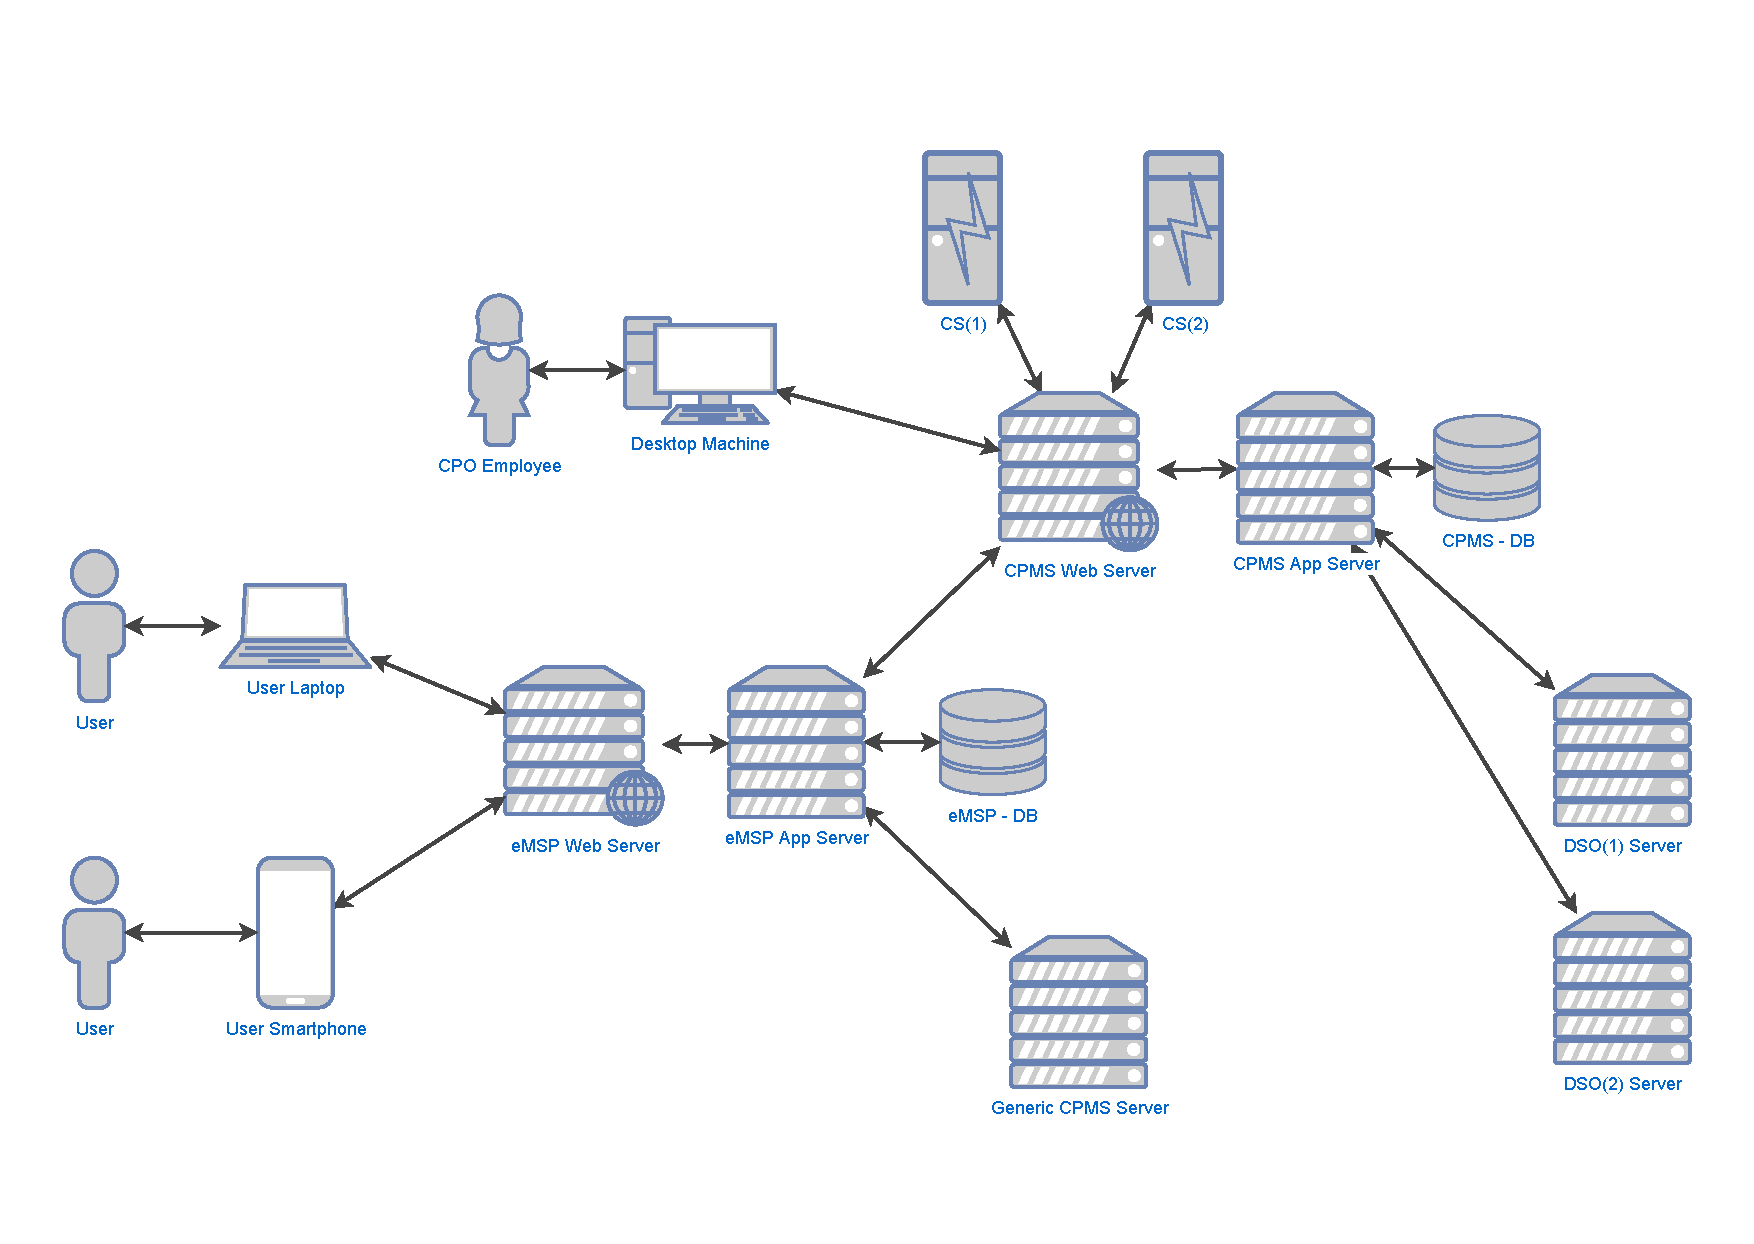
\includegraphics[page={1}, trim=1cm 1.25cm 1cm 1.25cm, width=\linewidth, clip]{OverviewDiagram.pdf}
    \caption{Overview Diagram}
\end{figure}

\begin{itemize}
    \item \textbf{eMSP Web Application} \\
        A Web Application that runs within the User’s web browser and that gives them access to the eMall services. All the resources it needs get downloaded to the User's browser from the eMSP Web Server as the the device reaches it through HTTP requests.
    \item \textbf{eMSP Web Server} \\
        Back-end component that interfaces the User's web browser with the other application services in the eMSP's back-end. It handles HTTP requests arriving from user-devices by routing them to the corresponding components that can respond to them.
    \item \textbf{eMSP App Server} \\
        The principal back-end component for the eMSP, it contains all the modules that together offer all functionalities available via the eMSP. Requests are routed from the Web Server to the module capable handling them, the response is than sent from the App Server through the Web Server to the User's device. The App Server is also capable of accessing the eMSP DataBase and the external services needed for its functions.
    \item \textbf{eMSP DataBase Server} \\
        Component dedicated to data storage for the eMSP, it stores for instance the Users' credentials and bookings, to ensure its safety it can only be accessed by the eMSP's App Server.
    \item \textbf{CPMS Web Application} \\
        A Web Application meant for the desktop devices available to CPO Employees, it runs withing the browser and allows its users to access the management functions of the CPMS. It dialogues with the CPMS Web Server through the HTTP protocol.
    \item \textbf{CPMS Web Server} \\
        Back-end component that interfaces the CPO Employees' web browser and the back-ends of the eMSP with the application services in the CPMS's back-end. It handles HTTP requests arriving from the outside by routing them to the corresponding components that can respond to them and allows tunneling of WebSocket connections from CS to the back-end.
    \item \textbf{CPMS App Server} \\
        The principal back-end component for the CPMS, it contains all the modules that together offer all functionalities available to the CPO and eMSPs, as well as being the endpoint where CS connect to in order to be managed. Requests and connections are routed from the Web Server to the module capable handling them, in the fist case the response is than sent from the App Server through the Web Server to the requesting device, in the second case the connection is handled and kept alive by its target module. The App Server is also capable of accessing the CPMS DataBase and the external services needed for its functions.
    \item \textbf{CPMS DataBase Server} \\
        Component dedicated to data storage for the CPMS, it stores for instance the credentials for CPO Employees as well as a local copy of the CSs' configurations, to ensure its safety it can only be accessed by the CPMS's App Server.
    \item \textbf{CS} \\
        External entity w.r.t. the STB, it is configured to reach out to the CPMS App Server via a WebSocket connection that allows the CPMS to manage and monitor it.
    \item \textbf{DSO} \\
        External entity w.r.t. the STB, it exposes a web API that allows CPMSs to acquire information regarding its price and energy mix.
    \item \textbf{Maps Provider} \\
        External entity w.r.t. the STB, offers to clients up to date maps of any requested area, as well as related information such as satellite images.
\end{itemize}

\subsection{Component View}

In this section, every major component is analysed in terms of its sub-components. \\
Everything that is outside of the system is considered as a black box.

\newpage

\begin{figure}[!ht]
    %trim = left bottom right top
    \centerline{
        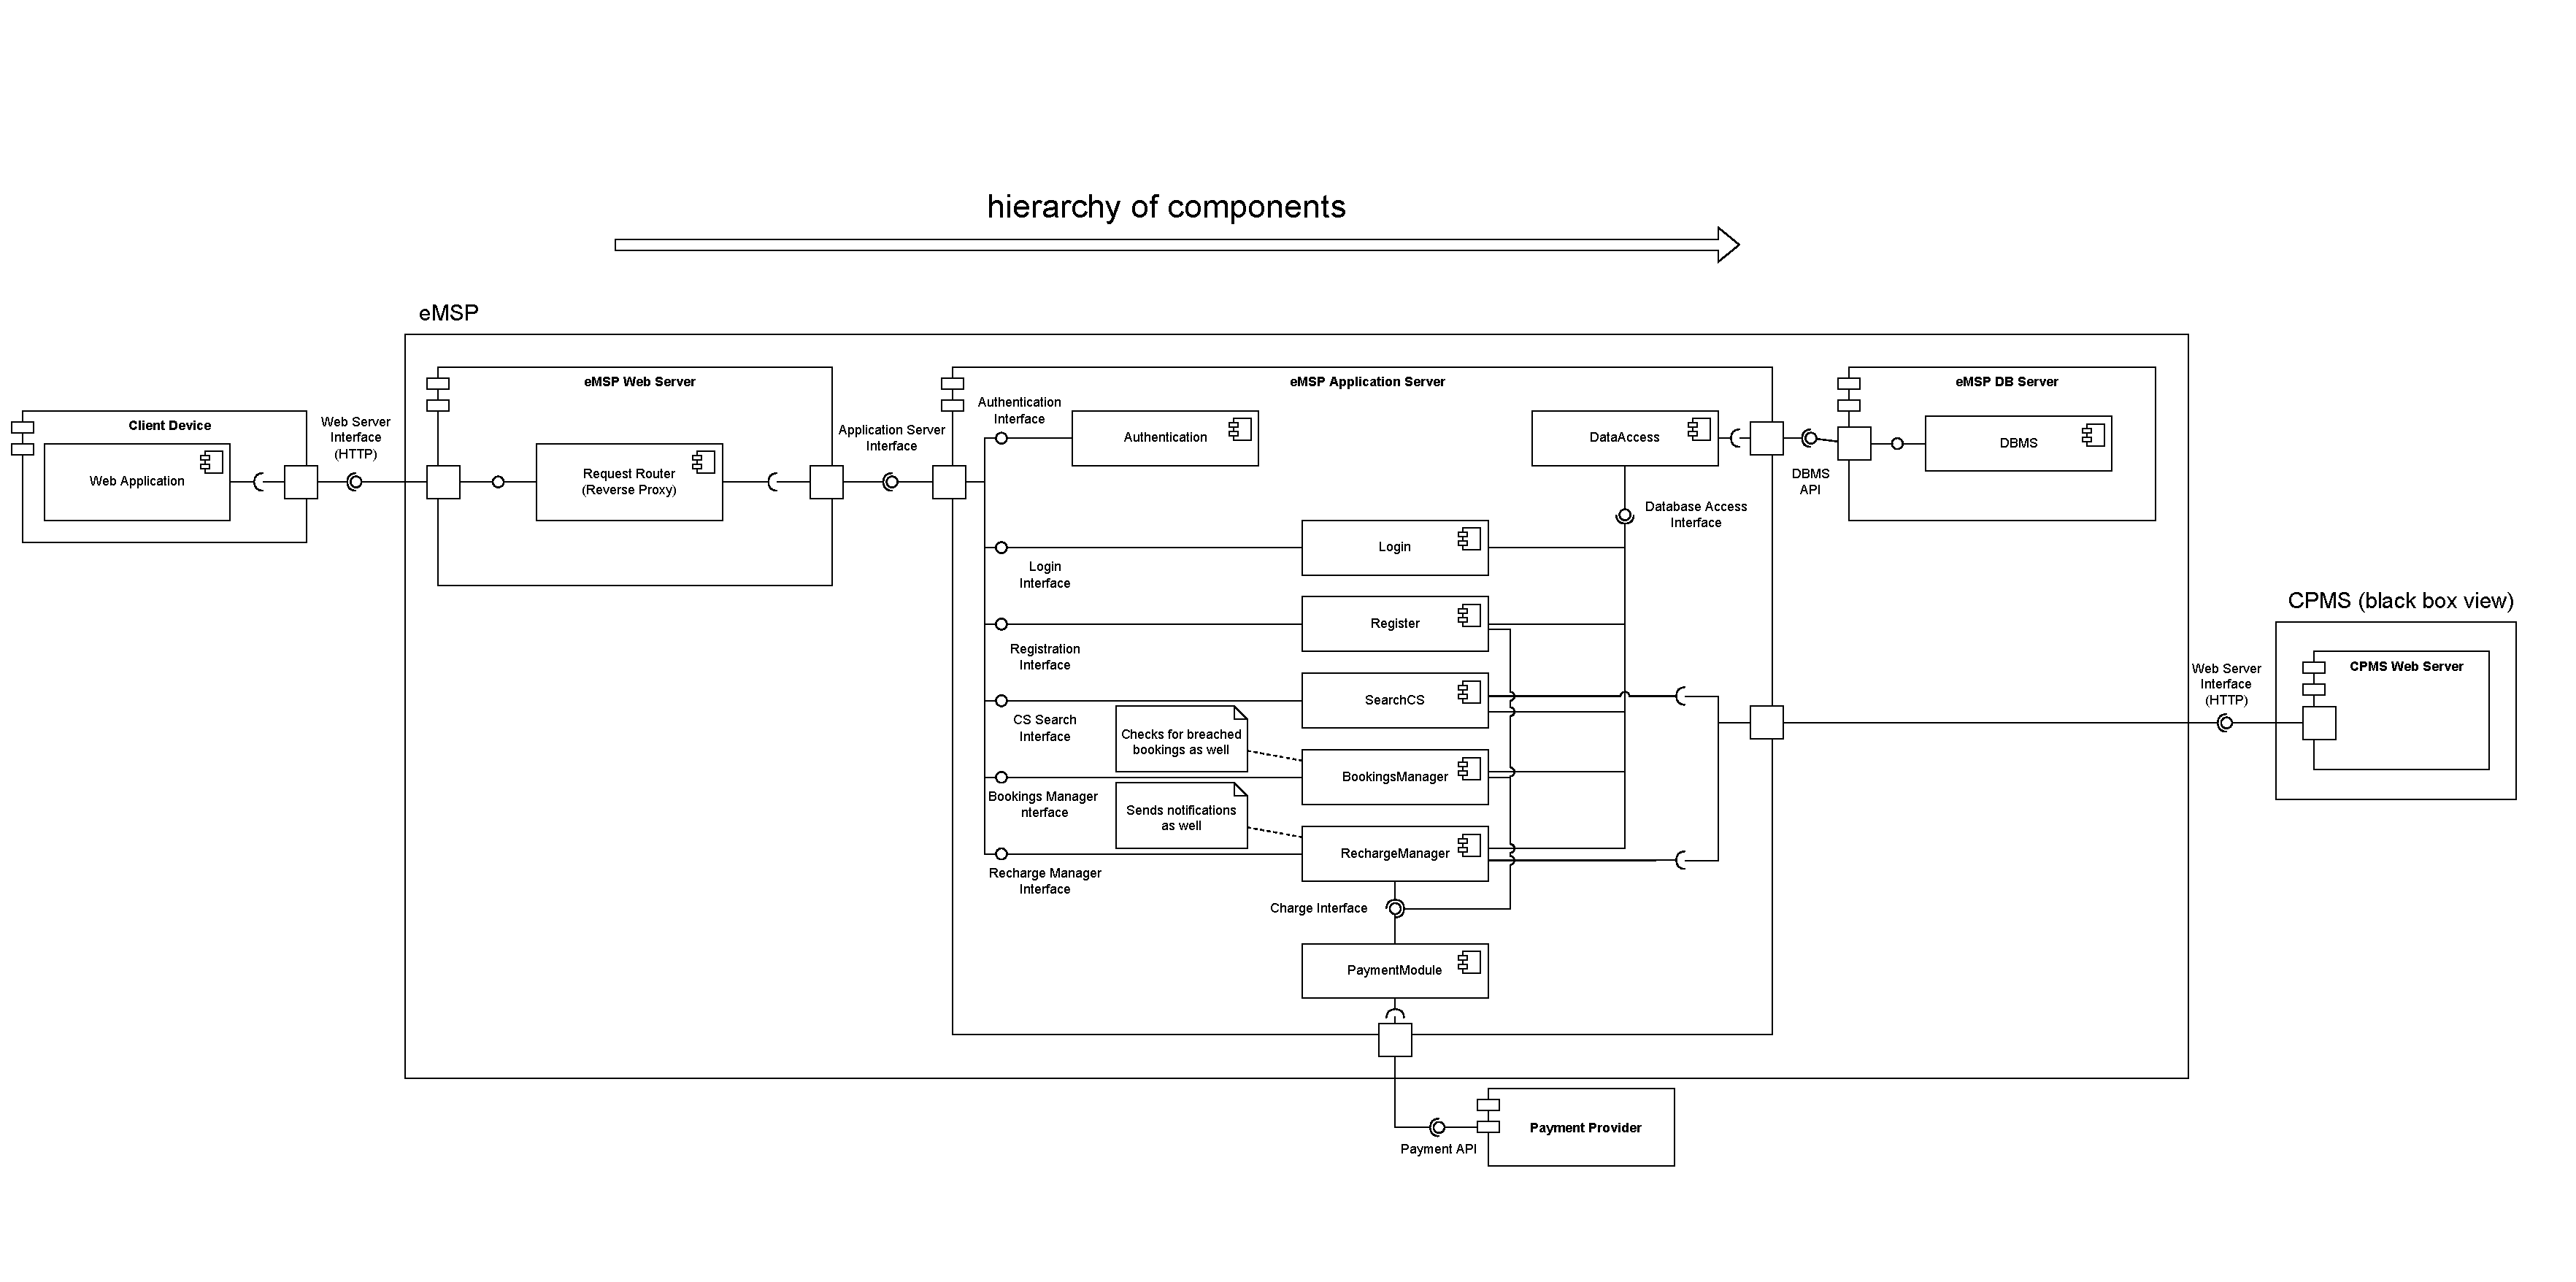
\includegraphics[page={1}, width=1.26\linewidth, trim=0cm 2cm 0cm 4cm, angle=-90, clip]{ComponentDiagram.pdf}
    }
    \caption{Component diagram}
\end{figure}

\newpage

\begin{figure}[!ht]
    %trim = left bottom right top
    \centerline{
        \includegraphics[page={2}, width=1.26\linewidth, trim=3cm 1cm 4cm 3cm, angle=-90, clip]{ComponentDiagram.pdf}
    }
    \caption{Component diagram}
\end{figure}

\newpage

\subsubsection{Client Device}

Client devices represent all the devices connected to the internet and used to reach the eMall website. By reaching eMall the \textbf{eMSP Web Application Component} in the form of an interactive web application is loaded by the device's web browser and eMall's UI is shown to the User.\\
\\
The \textbf{eMSP Web Application Component} is the front-end that it offers to its Users, it consists of a website offering an interactive web application with a UI that allows Users to access every function offered by eMall. This component does not integrate computational intensive tasks and in itself does not have any data that can instead be provided by eMall's back-end. Its functionalities are limited to error checking, UI rendering and contacting the eMSP's back-end to recover any data needed to offer the User the intended functionalities.

\subsubsection{eMSP Web Server Component}

The eMSP Web Server is required in order to serve the eMSP Web Application to User, and to allow such Web App to interact with the eMSP's back-end when needed. \\
\\
To this end its main sub-component is a \textbf{Request Router}, a Reverse Proxy component that sits in front of the back-end and routes requests from client devices to the back-end services capable of satisfying them, this way the resources returned to clients appear as if they originated from the Web Server itself. \\
The role of the Reverse Proxy is also to help increase scalability, performance, resilience and security by both acting as a content cache and as a middleware before the back-end. 

\subsubsection{eMSP Application Server Component}

The back-end for the eMSP, as per the hierarchy of components, every request reaching it is first checked for an active session, and only those with one which has a performed valid login are allowed access to components other than \textbf{Register}. \\
Every component present performs all the required checks on the received data to correctly perform any of its functions.

\begin{itemize}
    \item \textbf{Authentication} \\
        Sub-component that handles the authentication by checking the credentials for every request reaching the back-end.
    \item \textbf{Login} \\
        Sub-component which checks the login credentials inserted by Users through the Web App and grants them an authenticated session if those are valid.
    \item \textbf{Register} \\
        Sub-component that allows Unregistered Users to create a new account with eMall.
    \item \textbf{SearchCS} \\
        Sub-component whose purpose is to allow authenticated Users to query eMall for the CSs it has available with the use of filters. It returns the list of matching CSs.
    \item \textbf{BookingsManager} \\
        Sub-component offering the functionalities to both create a new booking and receive the current list of bookings for the authenticated User, with the possibility of deleting any booking. 
    \item \textbf{RechargeManager} \\
        Sub-component which allows for control over a booking which is currently active, after a User has connected their vehicle to a booked CS, via this component they can start/stop the charging process as well as get notified of the process terminating.
    \item \textbf{PaymentModule} \\
        Sub-component that interfaces with an external payment provider and allows the eMSP to charge Users for any obtained service or fee if they were not to show up for a booking.
    \item \textbf{DataAccess} \\
        Sub-component that provides access to the DataBase for every other sub-component.
\end{itemize}

\subsubsection{CPO Device}

CPO Devices represent all the machines available to CPO Employees to operate with the company's CPMS. \\
\\
The \textbf{CPMS Web Application Component} is meant to be ran inside a web browser on the CPO Devices and consequently be available to CPO Employees, it is the front-end offered by the CPMS and its UI is meant to offer to its users all the management functionalities of the CPMS. This component does not integrate computational intensive tasks and does not store locally any data that can instead be provided by the CPMS's back-end. Its functionalities are limited to error checking, UI rendering and contacting the CPMS's back-end to recover any data required for its functionalities.

\subsubsection{CPMS Web Server Component}

The CPMS Web Server is required in order to serve the CPMS Web Application to CPO Employees, to allow such Web App to interact with the CPMS's back-end and to allow CS to reach the CPMS with a WebSocket connection, allowing the CPMS to actively manage them. \\
\\
To this end its main sub-components are:

\begin{itemize}
    \item \textbf{Request Router} \\
        A reverse proxy that sits between a client and the CPMS back-end, its role is to route requests from clients to the back-end services capable of answering them, this way the resources resources returned to clients appear as if they originated from the Web Server itself. The role of the Reverse Proxy is also to help increase scalability, performance, resilience and security by both acting as a content cache and as a middleware before the back-end.
    \item \textbf{WebSocket Proxy} \\
        Its role is to tunnel WebSocket connections between the CPMS back-end and the CSs, after those are originated from upgrade requests over HTTP that went through the Request Router.
\end{itemize}

\subsubsection{CPMS Application Server Component}

The back-end for the CPMS, every request reaching it is let through to the CPO-only components only if it has an active authenticated session with CPO credentials. Access to components that are meant for eMSPs is granted to all eMSPs that are known by the system as long as their request are correctly performed with an authenticated session. \\
Every component present performs all the required checks on the received data to correctly perform any of its functions.

\begin{itemize}
    \item \textbf{Authentication} \\
        Sub-component that handles the authentication by checking the credentials for every request reaching the back-end.
    \item \textbf{Login} \\
        Sub-component which checks the login credentials inserted by CPO Employees through the Web App and grants them an authenticated session if those are valid.
    \item \textbf{CSBatteryPolicyManager} \\
        Sub-component that allows CPOs to change the policy currently in use by a CS to manage its batteries, it both saves to the CPMS's DataBase updated CS policies as well as requests the \textbd{CSManager} to communicate the updated policies to the actual CS.
    \item \textbf{CSDSOManager} \\
        Sub-component that allows CPOs to change the DSO currently supplying a CS, it both saves to the CPMS's DataBase updated CS's DSO as well as requests the \textbd{CSManager} to communicate the change to the actual CS.
    \item \textbf{CSPricesManager} \\
        Sub-component that allows CPOs to change the user-price, the nominal-price and the offer reset date of a CS, it both saves to the CPMS's DataBase updated prices and date as well as requests the \textbd{CSManager} to communicate the updated values to the actual CS.
    \item \textbf{AutomaticModeManager} \\
        Sub-component which allows CPO Employees to toggle the operating mode of the CPMS from “Automatic Mode” to “Manual Mode” or vice-versa, as well as allowing the CPO to update the CPMS’s policy for “Automatic Mode”.
    \item \textbf{CSList} \\
        Sub-component providing the CPO and external eMSPs with the list of CS currently under the control of the CPMS. It also accepts filters to reduce the list of provided CSs. If they are requested, details regarding a specific CS can also be provided by this component.
    \item \textbf{RechargeManager} \\
        Sub-component providing external eMSPs with the possibility of managing, on behalf of their Users, the ongoing charging process to a certain socket of a CS. This module also provides the eMSP feedback on the current status of the charging process. This component dialogues with the \textbd{CSManager} to gather the CS status and forward it commands to manage the charging process.  
    \item \textbf{DSOInformation} \\
        Sub-component providing the CPO with information regarding the DSOs known by the CPMS. This module also interfaces directly with the DSOs external API to gather their prices and energy mixes. 
    \item \textbf{CSManager} \\
        Sub-component that allows the other back-end components to dialogue with CSs, know their real-time status, coordinate their charging processes and update their configuration. CS signal this module when one of their recharges is complete, and this module forwards such notification to the eMSP. This module also accepts WebSocket connections from CS to allow their management.
    \item \textbf{DataAccess} \\
        Sub-component that provides access to the DataBase for every other sub-component.
\end{itemize}

\newpage

\subsubsection{eMSP DataBase Components}

SQL DataBase for the eMSP, it contains the accounts and bookings of all users.

%trim = left bottom right top
\begin{figure}[!ht]
    \centering
    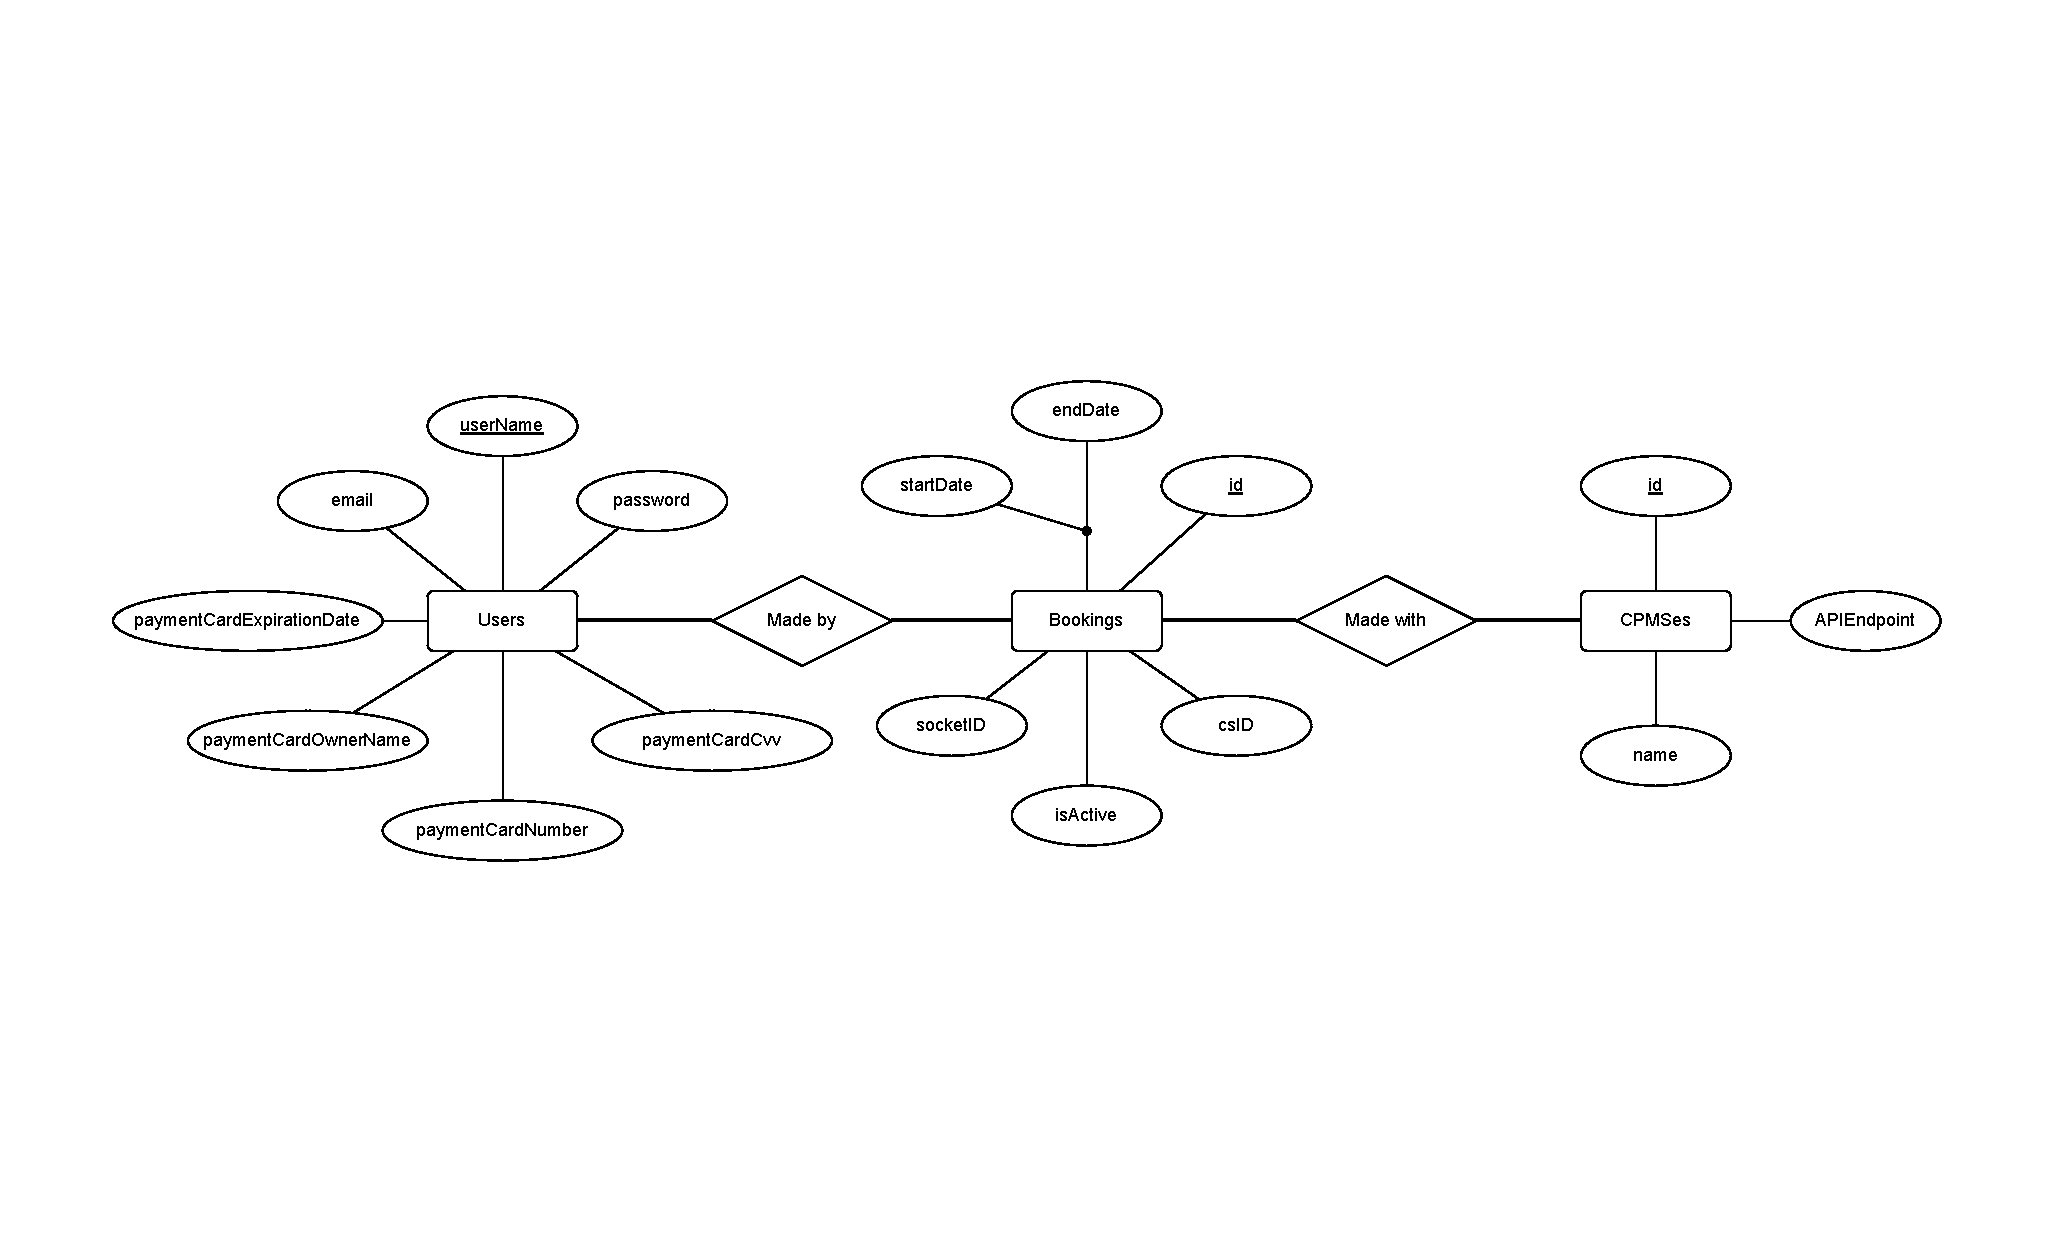
\includegraphics[page={1}, trim=1.5cm 6cm 1.5cm 6cm, width=\linewidth, clip]{ERDiagrams.pdf}
    \caption{eMSP ER Diagram}
\end{figure}

\subsubsection{CPMS DataBase Components}

SQL DataBase for the CPMS, it contains information on all known CSs and their configurations.

%trim = left bottom right top
\begin{figure}[!ht]
    \centering
    \includegraphics[page={2}, trim=5cm 3.5cm 5cm 3.5cm, width=\linewidth, clip]{ERDiagrams.pdf}
    \caption{CPMS ER Diagram}
\end{figure}

\newpage

\subsubsection{External Systems}

Systems outside the scope of this document, whose existence is acknowledge in order to explain the behaviour of certain components of the STB.

\begin{itemize}
    \item \textbf{DSO} \\
        An endpoint with an exposed API that allows for retrieval of information regarding the DSO's energy mix and prices.
    \item \textbf{Payment Provider} \\
        An endpoint that allows, given adequate payment details, to charge someone for a service and move the sum to a certified bank account.
    \item \textbf{Map Provider} \\
        A service providing up to date maps for the entire world. It is reached by the eMSP Web Application to improve the UI with an interactive map.
\end{itemize}

\newpage

\subsection{Deployment View}

Here we describe the arrangement of physical nodes and the components deployed on them. \textbf{Load balancers} and \textbf{Firewalls} are also included in the diagram:
\begin{itemize}
    \item \textbf{Firewall} \\
        Is directly connected to the Internet and filters incoming packets, only letting pass those identified as trustworthy.
    \item \textbf{Load balancer} \\
        A device that forwards requests to the back-end's services in accordance to their current load, aiming to distribute work evenly. Its presence improves the maximum load capacity the system can handle and its reliability. 
\end{itemize}

%trim = left bottom right top
\begin{figure}[!ht]
    \centering
    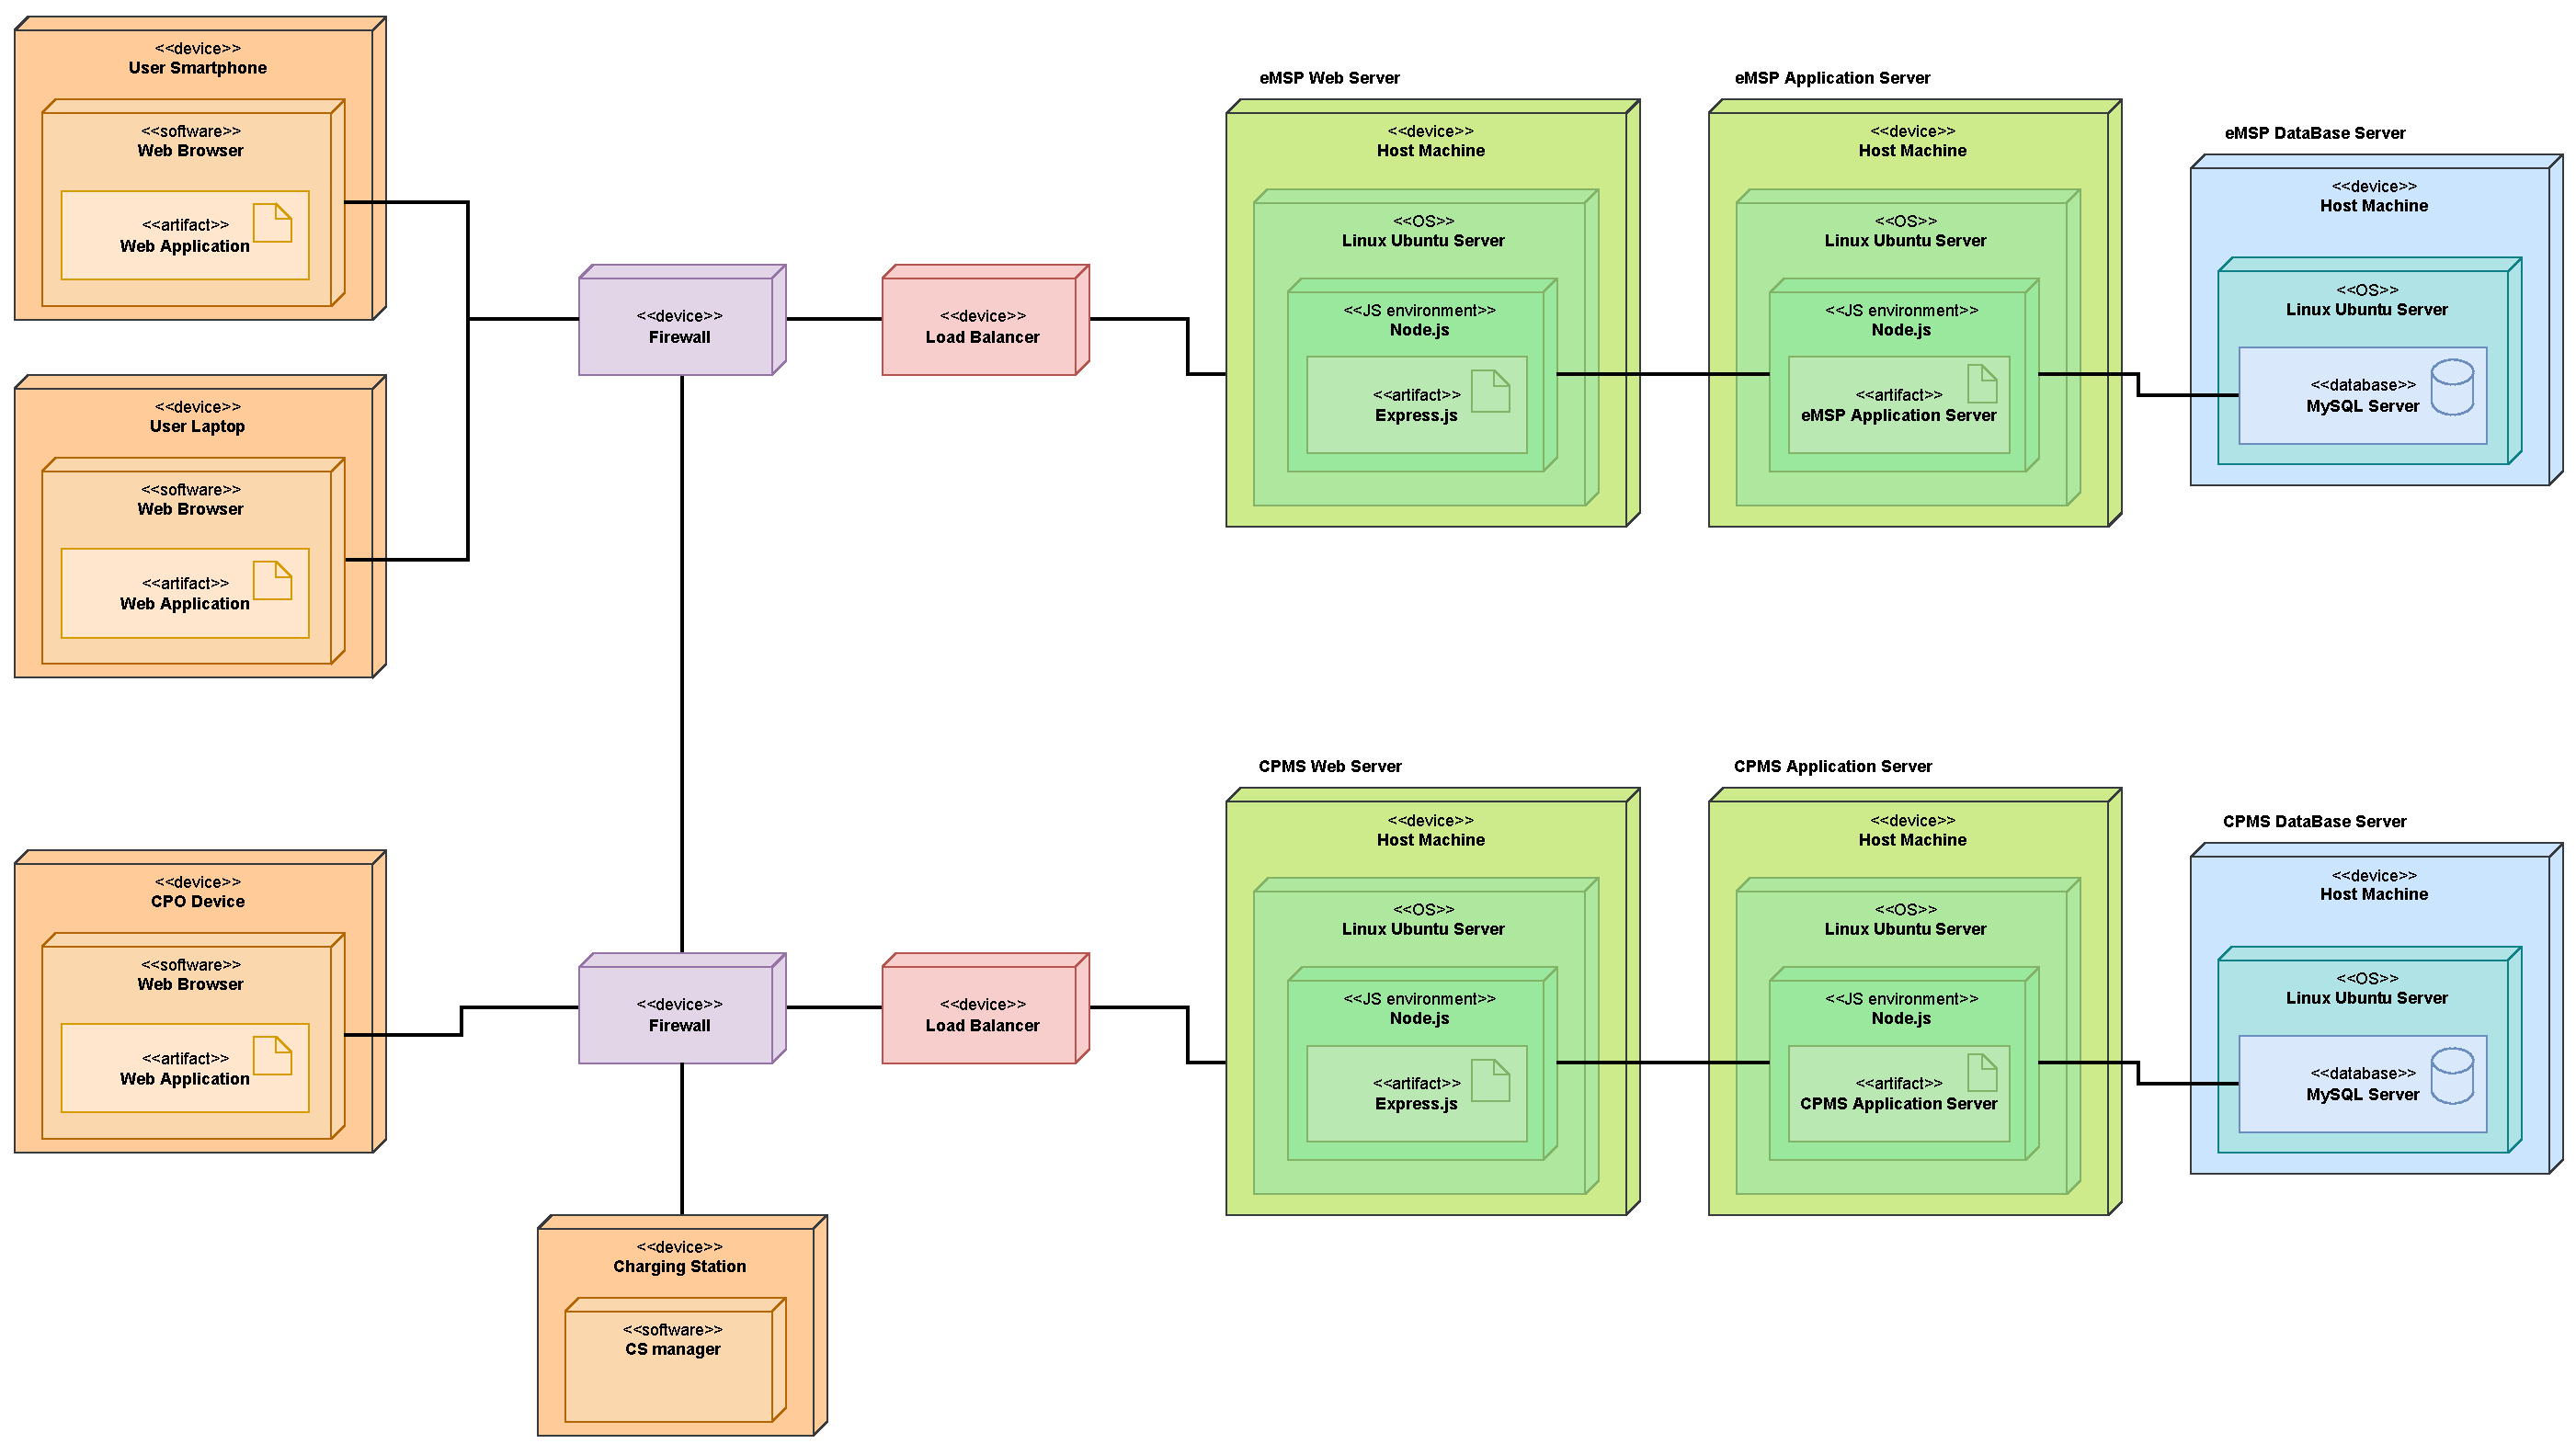
\includegraphics[page={1}, trim=0cm 0cm 0cm 0cm, width=\linewidth, clip]{DeploymentView.pdf}
    \caption{Deployment View}
\end{figure}
    
Client devices will only need to reach the Web Server of the eMSP, which will then forward their requests to the eMSP's back-end if needed.

\newpage

\subsection{Runtime View}

In this section the dynamic behaviour of the system is presented via sequence diagrams that summarize all the possible interactions that can be had with both the eMSP or the CPMS. Each diagram further expands on those discussed in the RASD document in section 3.2.3 .

\begin{description}
    \item \textbf{1. New user registration}
    %trim = left bottom right top
    \begin{figure}[!ht]
        \centering
        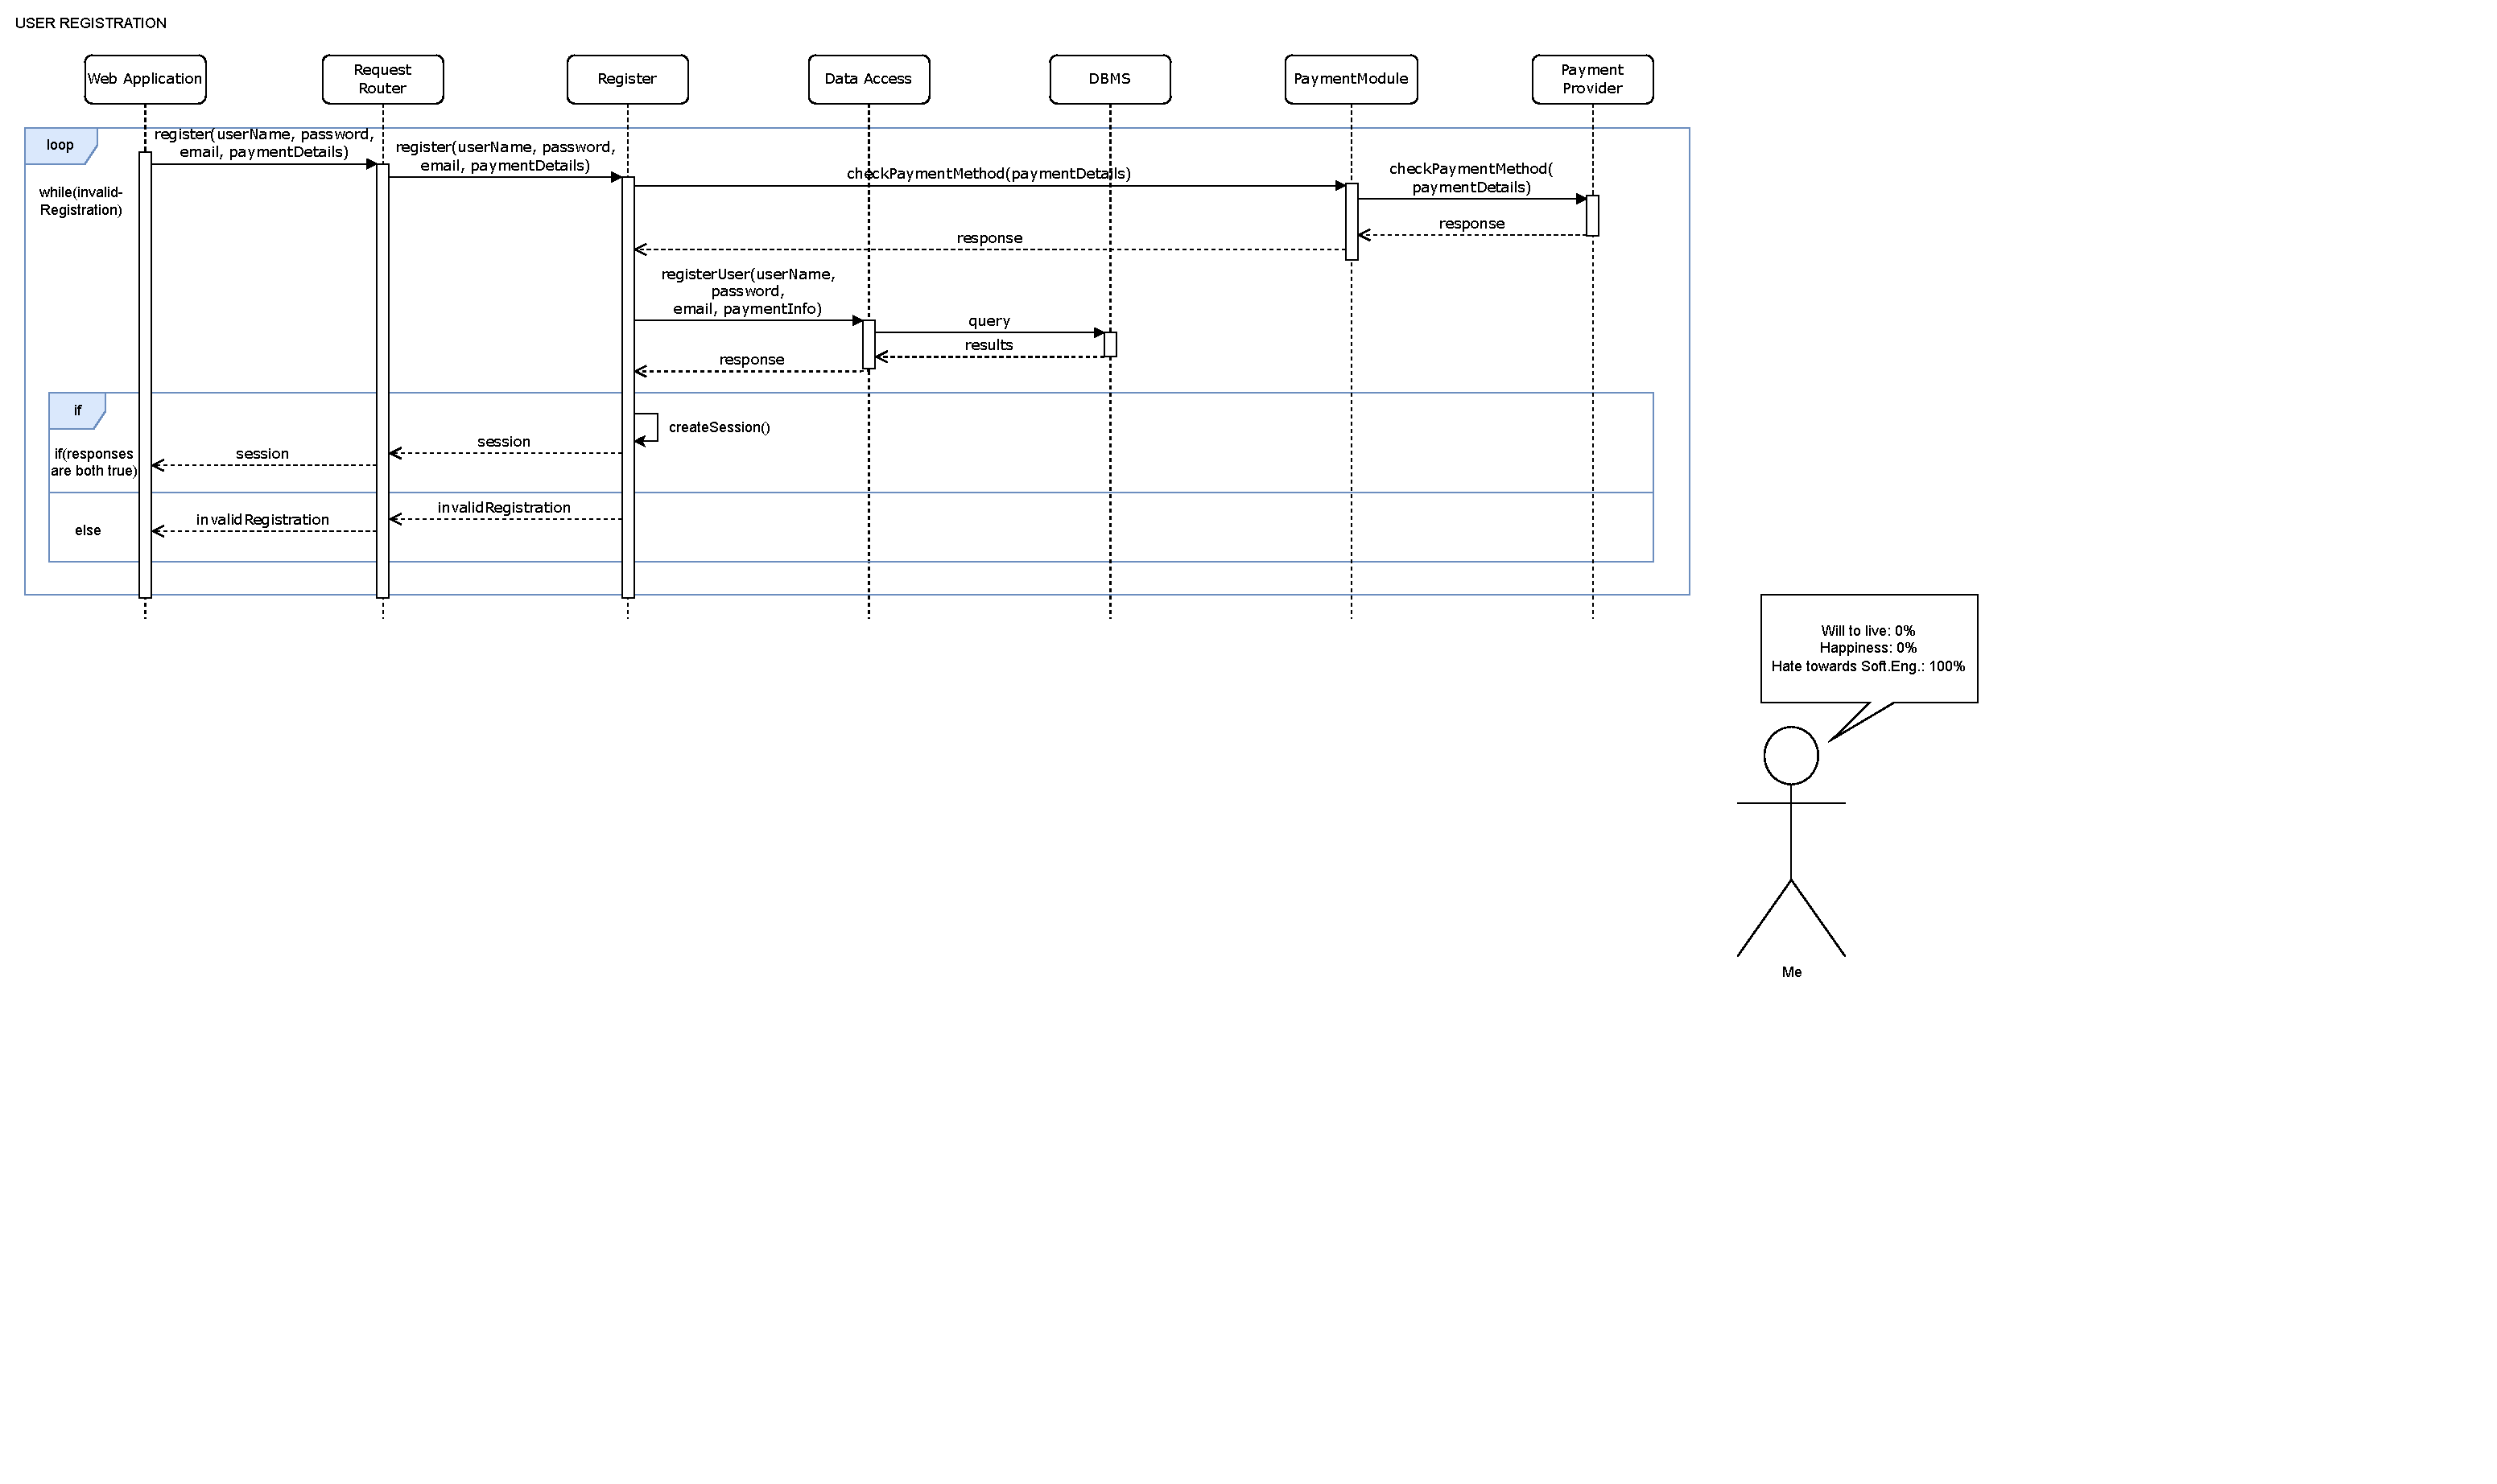
\includegraphics[page={1}, trim=0cm 18cm 16cm 1cm, width=\linewidth, clip]{RuntimeDiagrams.pdf}
        \caption{New user registration}
    \end{figure}
    
    \item \textbf{2. User login}
    %trim = left bottom right top
    \begin{figure}[!ht]
        \centering
        \includegraphics[page={2}, trim=0cm 20cm 25cm 1cmm, width=\linewidth, clip]{RuntimeDiagrams.pdf}
        \caption{User login}
    \end{figure}
    
    \newpage
    
    \item \textbf{3. User searching and booking a CS}
    %trim = left bottom right top
    \begin{figure}[!ht]
        \centering
        \includegraphics[page={3}, trim=0cm 5cm 0cm 1cmm, width=\linewidth, clip]{RuntimeDiagrams.pdf}
        \caption{User login}
    \end{figure}
    
    \item \textbf{4. User deleting one of his bookings}
    %trim = left bottom right top
    \begin{figure}[!ht]
        \centering
        \includegraphics[page={4}, trim=0cm 10cm 21cm 1cmm, width=0.95\linewidth, clip]{RuntimeDiagrams.pdf}
        \caption{User deleting one of his bookings}
    \end{figure}
    
    \newpage
    
    \item \textbf{5. User starting a charging process}
    %trim = left bottom right top
    \begin{figure}[!ht]
        \centering
        \includegraphics[page={5}, trim=0cm 7cm 8cm 1cmm, width=\linewidth, clip]{RuntimeDiagrams.pdf}
        \caption{User starting a charging process}
    \end{figure}
    
    \item \textbf{6. User interrupting a charging process}
    %trim = left bottom right top
    \begin{figure}[!ht]
        \centering
        \includegraphics[page={6}, trim=0cm 3cm 1cm 1cmm, width=\linewidth, clip]{RuntimeDiagrams.pdf}
        \caption{User interrupting a charging process}
    \end{figure}
    
    \newpage
    
    \item \textbf{7. Charging procedure self-terminates and User receives a notification}
    %trim = left bottom right top
    \begin{figure}[!ht]
        \centering
        \includegraphics[page={7}, trim=0cm 16cm 0cm 1cmm, width=\linewidth, clip]{RuntimeDiagrams.pdf}
        \caption{Charging procedure self-terminates and User receives a notification}
    \end{figure}
    
    \item \textbf{8. User does not show up for a booked recharge}
    %trim = left bottom right top
    \begin{figure}[!ht]
        \centering
        \includegraphics[page={8}, trim=0cm 19cm 26cm 1cmm, width=0.8\linewidth, clip]{RuntimeDiagrams.pdf}
        \caption{User does not show up for a booked recharge}
    \end{figure}
    
    \item \textbf{9. CPO logs in into the CPMS}
    %trim = left bottom right top
    \begin{figure}[!ht]
        \centering
        \includegraphics[page={9}, trim=0cm 20cm 25cm 1cmm, width=0.95\linewidth, clip]{RuntimeDiagrams.pdf}
        \caption{CPO logs in into the CPMS}
    \end{figure}
    
    \newpage
    
    \item \textbf{10. CPO retrieves energy prices and mixes from DSOs}
    %trim = left bottom right top
    \begin{figure}[!ht]
        \centering
        \includegraphics[page={10}, trim=0cm 17cm 25cm 1cmm, width=\linewidth, clip]{RuntimeDiagrams.pdf}
        \caption{CPO retrieves energy prices and mixes from DSOs}
    \end{figure}
    
    \newpage
    
    \item \textbf{11. CPO assigns nominal-price, user-price, energy sources and battery usage policies for a CS} \\
    %trim = left bottom right top
    \begin{figure}[!ht]
        \centering
        \includegraphics[page={11}, trim=0cm 4cm 1cm 1cm, width=\linewidth, clip]{RuntimeDiagrams.pdf}
        \caption{CPO assigns nominal-price, user-price, energy sources and battery usage policies for a CS}
    \end{figure} \\
    This diagram summarized 3 views in one, by simply substituting the following components and interactions to the $\ast s$ one can obtain the different versions:
    \begin{enumerate}
        \item \textbf{CPO assigns nominal-price, user-price}
        \begin{description}
            \item $\ast\ \rightarrow$ CSPricesManager
            \item $\ast\ast \rightarrow$ updateCSPrices(CSID, userprice, nominalprice)
            \item $\ast\ast\ast \rightarrow$ updateCSPrices(userprice, nominalprice)
        \end{description}
        \item \textbf{CPO assigns energy sources}
        \begin{description}
            \item $\ast \rightarrow$ CSDSOManager
            \item $\ast\ast \rightarrow$ updateCSDSO(CSID, DSOId)
            \item $\ast\ast\ast \rightarrow$ updateCSDSO(DSOId)
        \end{description}
        \item \textbf{CPO assigns energy battery usage policies}
        \begin{description}
            \item $\ast \rightarrow$ CSBatteryPolicyManager
            \item $\ast\ast \rightarrow$ updateCSBatteryPolicy(CSID, thresholds, weights)
            \item $\ast\ast\ast \rightarrow$ updateCSBatteryPolicy(thresholds, weights)
        \end{description}
    \end{enumerate}
    
    \newpage
    
    \item \textbf{12. CPO toggles the CPMS operating mode}
    %trim = left bottom right top
    \begin{figure}[!ht]
        \centering
        \includegraphics[page={12}, trim=0cm 16cm 28cm 1cmm, width=0.95\linewidth, clip]{RuntimeDiagrams.pdf}
        \caption{CPO toggles the CPMS operating mode}
    \end{figure}
    
    \item \textbf{13. CPO changes the CPMS’s “Automatic Mode” policy}
    %trim = left bottom right top
    \begin{figure}[!ht]
        \centering
        \includegraphics[page={13}, trim=0cm 15cm 27cm 1cmm, width=0.95\linewidth, clip]{RuntimeDiagrams.pdf}
        \caption{CPO CPO changes the CPMS’s “Automatic Mode” policy}
    \end{figure}
\end{description}

\newpage

\subsection{Component Interfaces}

\subsection{Selected Architectural Styles and Patterns}

\subsection{Other Design Decision}

\section{User Interface Design}

\section{Requirements Traceability}

\section{Implementation, Integration and Test Plan}

%Bottom-up

\section{Effort Spent}

\subsection{Ronzani Marco - mat: 224578}

\begin{tabular}{|l|l|}
    \hline
    \textbf{Task} & \textbf{Time spent} \\
    \hline
    Introduction & $\infty h$ \\
    \hline
    Architectural Design & $\infty h$ \\
    \hline
    User Interface Design & $\infty h$ \\
    \hline
    Requirements Traceability & $\infty h$ \\
    \hline
    Implementation, Integration and Test Plan & $\infty h$ \\
    \hline
    Other & $\infty h$ \\
    \hline
    \hline
    Total & $5*\infty h$ \\
    \hline
\end{tabular}

\subsection{Sassi Alessandro - mat: ...}

\begin{tabular}{|l|l|}
    \hline
    \textbf{Task} & \textbf{Time spent} \\
    \hline
    Introduction & $\infty h$ \\
    \hline
    Architectural Design & $\infty h$ \\
    \hline
    User Interface Design & $\infty h$ \\
    \hline
    Requirements Traceability & $\infty h$ \\
    \hline
    Implementation, Integration and Test Plan & $\infty h$ \\
    \hline
    Other & $\infty h$ \\
    \hline
    \hline
    Total & $5*\infty h$ \\
    \hline
\end{tabular}

\newpage

\section{References}

\end{document}
